%% TITLE	Physiological Fluid Mechanics, Summary 4

%% AUTHOR	BINGHUAN W LI (Dept. Chemical Eng/Bio Eng, Imperial)
%%          PETER Y XIE (Dept. Mech Eng, Stanford)

%% compiled in XeLaTeX with Tex Live version 2023.

%% This work is licensed under a Creative Commons Attribution-NonCommercial 4.0 International License.

\documentclass[a4paper]{article}
\def\NotesType{1}
\def\summaryNo{4}
\def\finalise{1}
%% TITLE	Physiological Fluid Mechanics, configuration

%% DATE		- Nov 19, 2023     create

%% AUTHOR	BINGHUAN W LI (Dept. Chemical Eng/Bio Eng, Imperial)
%%          PETER Y XIE (Dept. Mech Eng, Stanford)

%% compiled in XeLaTeX with Tex Live version 2023.

%% This work is licensed under a Creative Commons Attribution-NonCommercial 4.0 International License.

\usepackage[sfdefault]{arimo}
\usepackage[left=1.5cm, right=1.5cm, top=2cm, bottom=1.5cm]{geometry}
\usepackage{amsmath, amsfonts, amssymb, cancel}
\usepackage{unicode-math}
\setmathfont
    [    Extension = .otf,
         BoldFont = XITSMath-Bold,
    ]{XITSMath-Regular}

% % \DeclareMathSizes{10}{12}{10}{9}

% \usepackage{siunitx}
\usepackage{enumitem}
\usepackage{xcolor}
    \definecolor{linkcolour}{rgb}{0,0.2,0.6}
\usepackage{hyperref}
\hypersetup{
    colorlinks,
    breaklinks,
    urlcolor=linkcolour,
    linkcolor=linkcolour,
    citecolor=black,
    pdfauthor={Li, Binghuan W},
    }
\usepackage{graphicx, float}
\usepackage{framed}
\usepackage[export]{adjustbox}

\usepackage{fancyhdr}
    \pagestyle{fancy}
    \fancyhf{}
    \lhead{\textsc{Physiological Fluid Mechanics Summary \summaryNo}}
    \rhead{page \thepage}

\usepackage{tcolorbox}

\usepackage{tikz, circuitikz}

\usepackage{multicol}
    \setlength{\columnseprule}{1pt}

\usepackage{lscape}

\usepackage{booktabs}

\usepackage{pifont}

\setlength\parindent{0pt}

\begin{document}

\section{Turbulence}
\paragraph{The Reynolds number} $\rm Re$ measures the ratio of the momentum force to the viscus force. For \textbf{tube} flow,
\[ 
    {\rm Re} = \frac{\rho UD}{\mu} = \frac{UD}{\nu}
    = \begin{cases}
        < 2000, & \text{laminar} \\
        2000 - 3000, & \text{transient} \\
        > 3000, & \text{turbulence}
    \end{cases}.
\]

\paragraph{Turbulence characteristics}
\begin{itemize}
    \item \textbf{Random variation} of fluid properties (\textit{e.g.}, pressure and velocities) in time and space. Each property has a specific continuous energy spectrum which drops to zero at high wave numbers;
    
    \item \textbf{Eddies} or fluid packets of many sizes, which intermingle and fill the shear layers down to the smallest scale (as defined by Kolmogorov);
    
    \item \textbf{Self-sustaining motion} – once triggered, turbulent flow can maintain itself by producing new eddies to replace those lost to viscous dissipation;
    
    \item \textbf{Mixing} – rapid convection of mass, momentum and energy, much stronger than laminar flows. 
\end{itemize}

\begin{figure}[H]
    \centering
    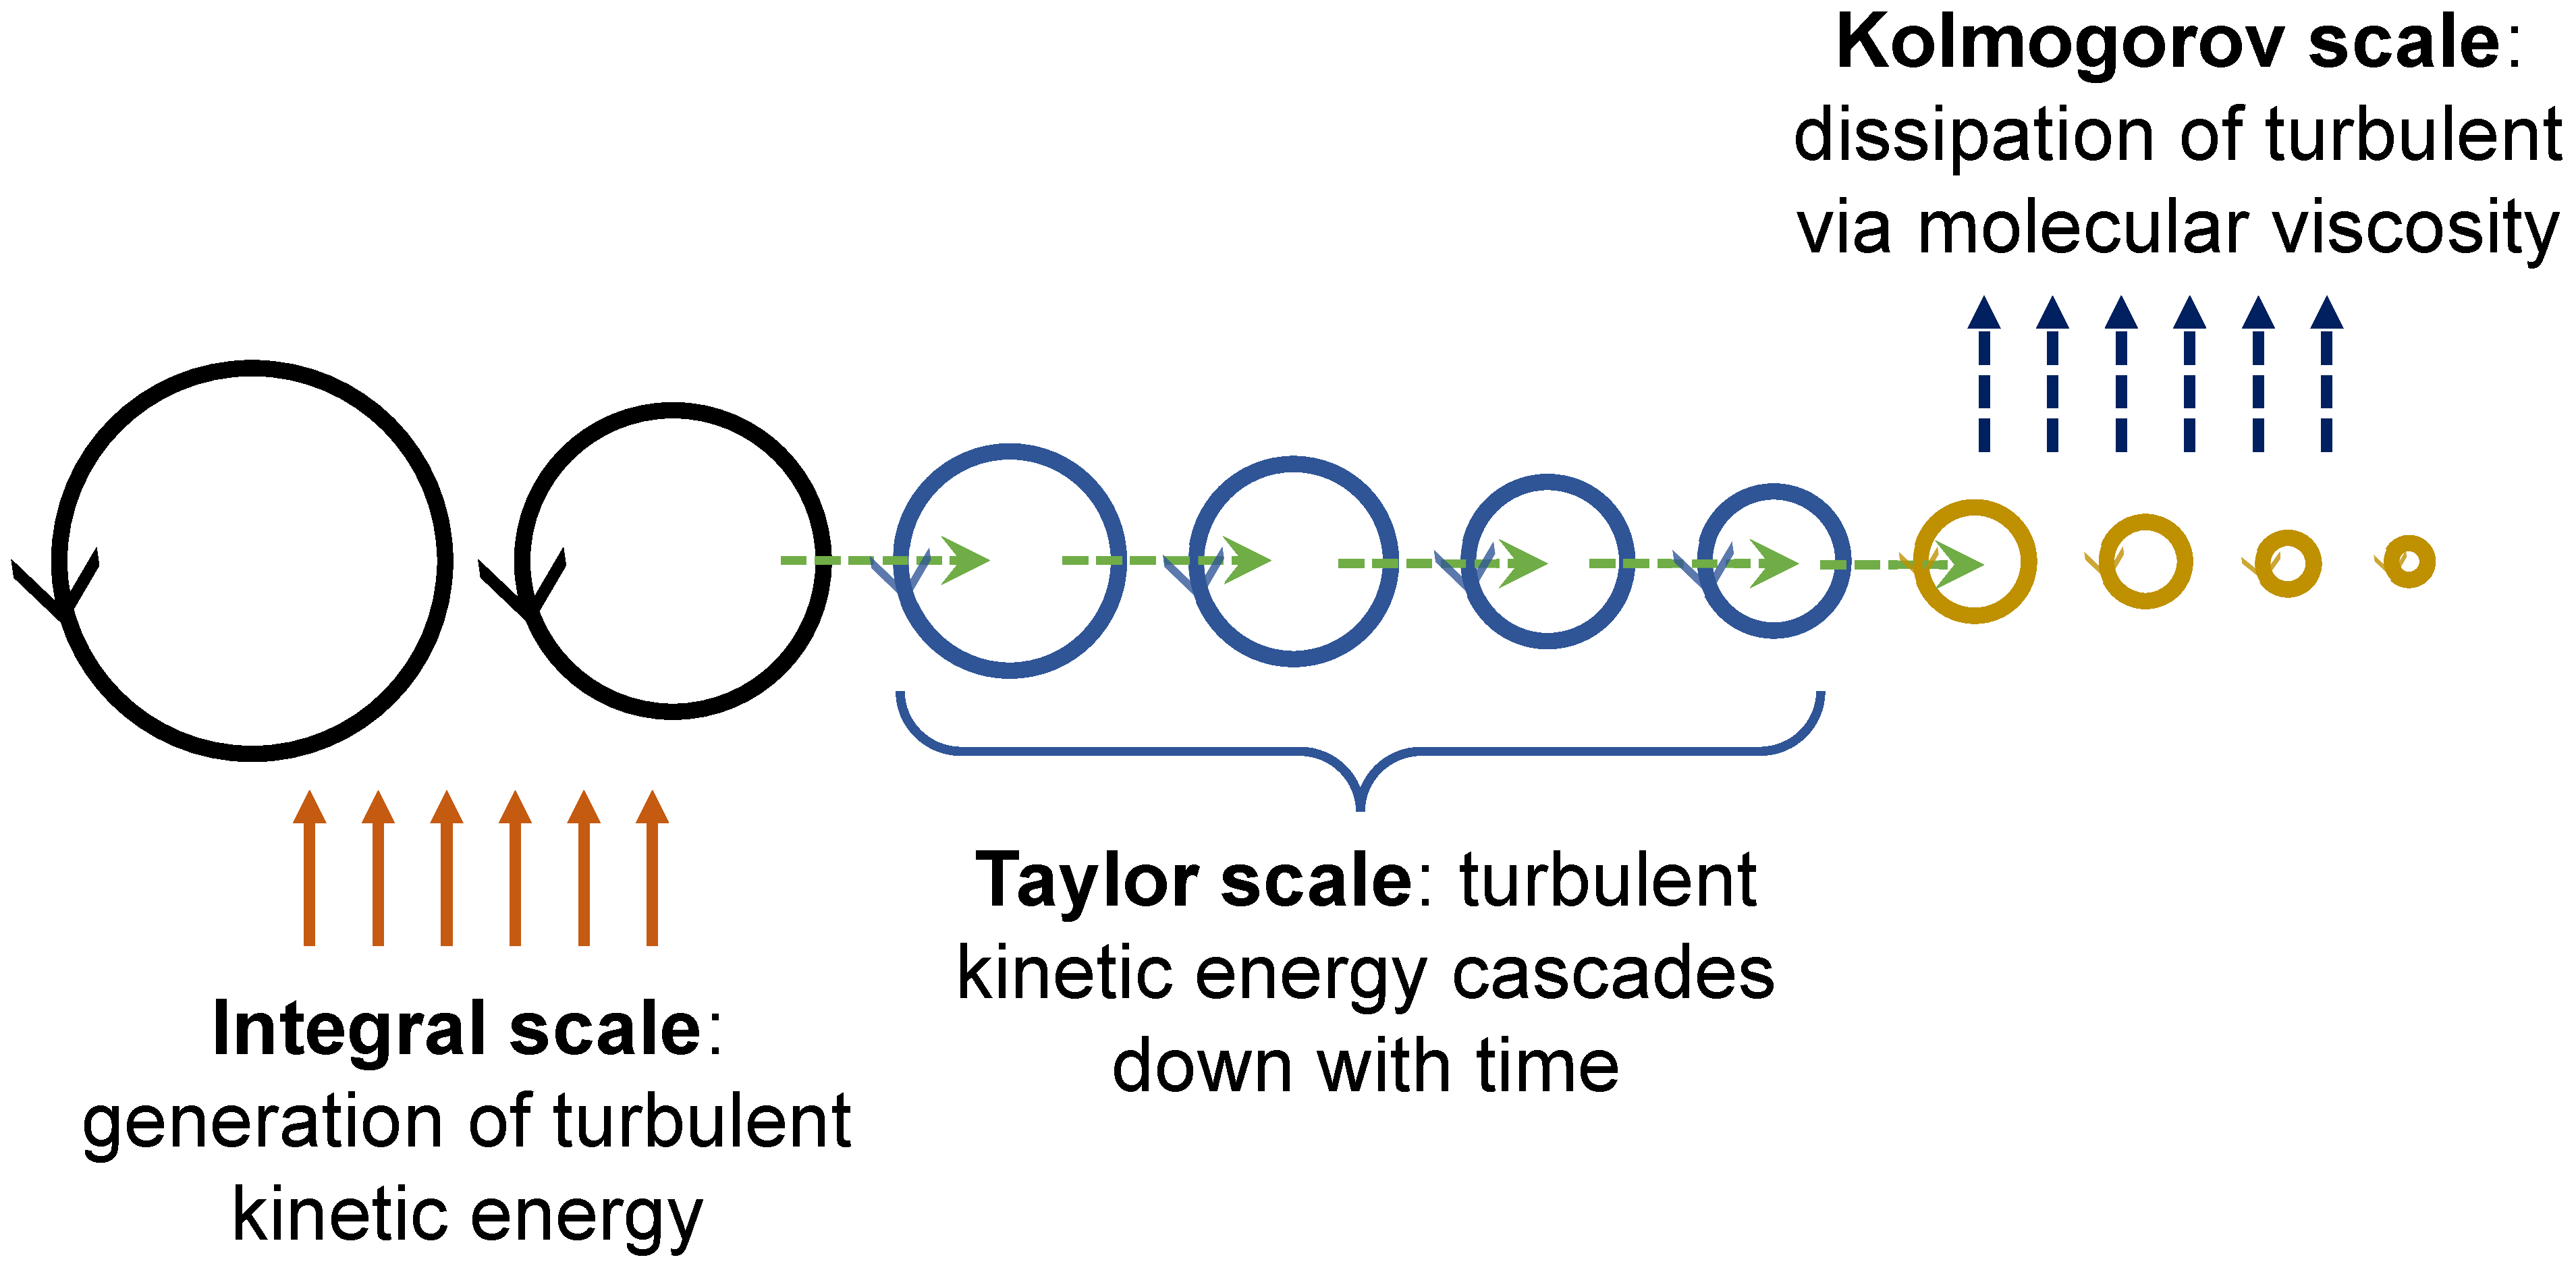
\includegraphics[width=.6\textwidth]{img/eddies.eps}
    \caption{Cascade of turbulence kinetic energy. The turbulence kinetic energy is generated on the integral scale (large eddies) and dissipated on the Kolmogorov scale (small eddies).}
\end{figure}

\paragraph{Reynolds averaging} Turbulence cannot be measured. It can only be \textit{characterised} in a \textit{statistical} manner by decomposing a certain flow quantity (\textit{e.g.}, velocity) into the mean and standard deviation (fluctuation) components. 
\[
    u(t) = \Bar{u} + u'(t).
\]

\begin{minipage}{.4\textwidth}
\vspace{.5cm}
\begin{center}
    \begin{tabular}{c c}
    \toprule
    average velocity    &   velocity fluctuation\\
    \midrule
    $\Bar{u} = \frac{1}{T} \int_{0}^{T} u \mathrm{d}t$     & $u' = u - \Bar{u}$\\
    \bottomrule
    \end{tabular}
\end{center}
\end{minipage}
\begin{minipage}{.6\textwidth}
    \begin{figure}[H]
        \centering
        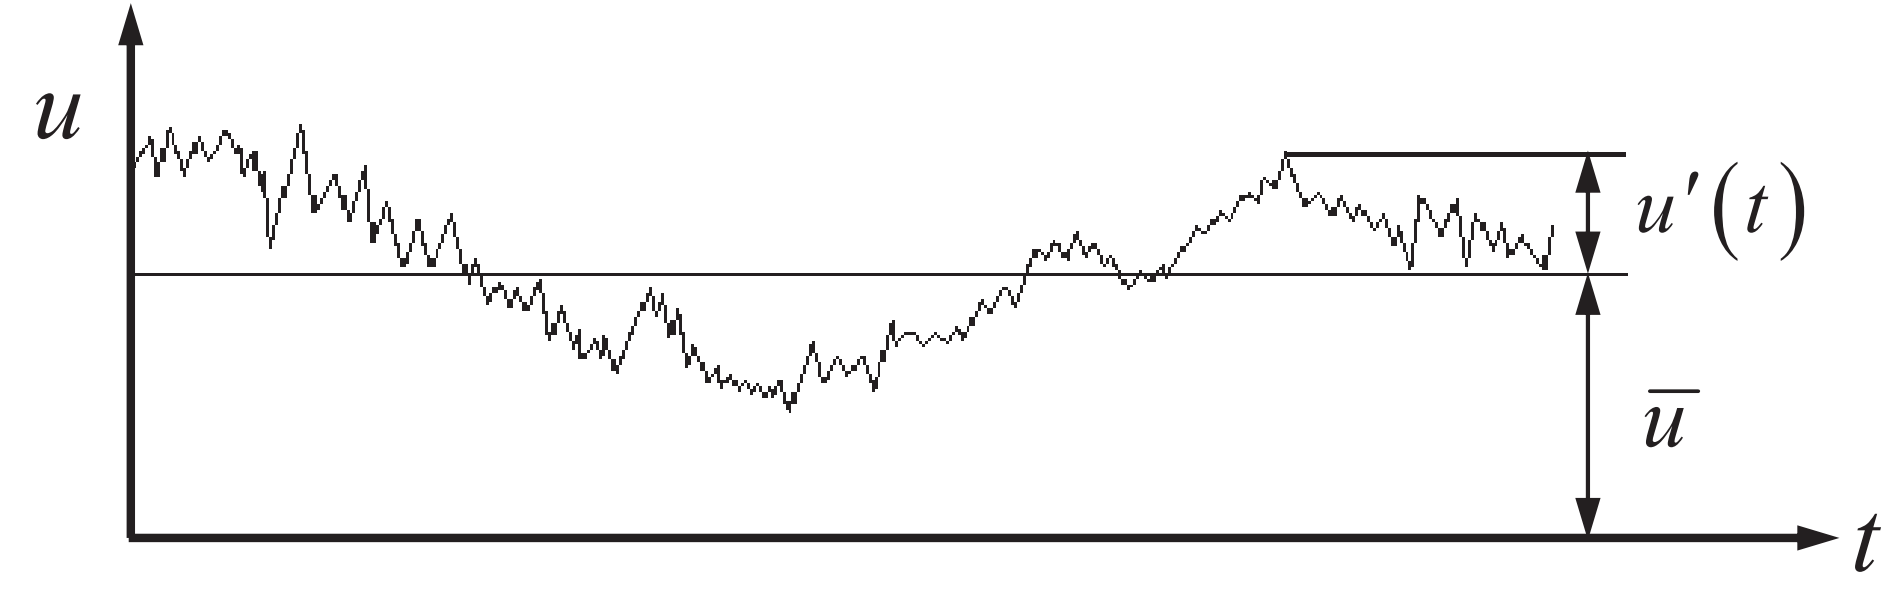
\includegraphics[width=.7\textwidth]{img/turbulence_v.PNG}
    \end{figure}
\end{minipage}

\vspace{.2cm}
Hence, the $x$-momentum equation becomes (similar for $y$- and $z$-momentum equations),
\[
    \rho \frac{D\Bar{u}}{Dt} = -\frac{\partial \Bar{p}}{\partial x} + \frac{\partial}{\partial x} \bigg(\mu \frac{\partial\Bar{u}}{\partial x} - \rho \overline{u'u'}\bigg) + \frac{\partial}{\partial y} \bigg(\mu \frac{\partial\Bar{u}}{\partial y} - \rho \overline{u'v'}\bigg) + \frac{\partial}{\partial z} \bigg(\mu \frac{\partial\Bar{u}}{\partial z} - \rho \overline{u'w'}\bigg) + \rho f_x,
\]
where the $\tau_{ij}' = \rho\overline{u_i' u_j'}$ terms are referred to as the \textbf{Reynolds stresses} (9 terms in total), which need to be resolved with appropriate turbulence closure methodologies (\textit{e.g.}, RANS $k$-$\varepsilon$ model subjected to the Boussinesq approximation).

%=================================================
\section{Energy Equation}
\paragraph{The Bernoulli equation} The Bernoulli equation assumes the fluid is incompressible and inviscid, the flow is steady, laminar, and no energy loss. It is applied between two points lying on the same streamline,
\[
    \frac{p_1}{\rho g} + \frac{1}{2g}u_1^2 + z_1 = \frac{p_2}{\rho g} + \frac{1}{2g}u_2^2 + z_2.
\]
The Bernoulli equation can be interpreted as the conservation of mechanical energy in \textit{frictionless} flow.

\paragraph{The pipe flow energy equation}
\[
    \frac{p_1}{\rho g} + \frac{1}{2g}u_1^2 + z_1 = \frac{p_2}{\rho g} + \frac{1}{2g}u_2^2 + z_2 + {\color{red} h_f},
\]
where $\displaystyle h_{f} = f\frac{L}{D}\frac{U^{2}}{2g}$, denotes the \textbf{major head loss}, is added to the Bernoulli equation. This term is the energy loss due to fluid friction, where $f$ is the Darcy friction factor. The presence of $h_f$ leads to the pressure drop: $\Delta p = h_f \rho g$.
\begin{itemize}
    \item For the flow in a circular pipe, if the flow is laminar (essentially, Poiseuille flow), $f = 64/{\rm Re}$;
    
    \item If the flow is turbulent, one needs to consult the Moody diagram, where the friction factor is related to the Reynolds number and the relative wall roughness of the pipe, $f\left({\rm Re}, \dfrac{\varepsilon}{d}\right)$.
\end{itemize}
\begin{figure}[H]
    \centering
    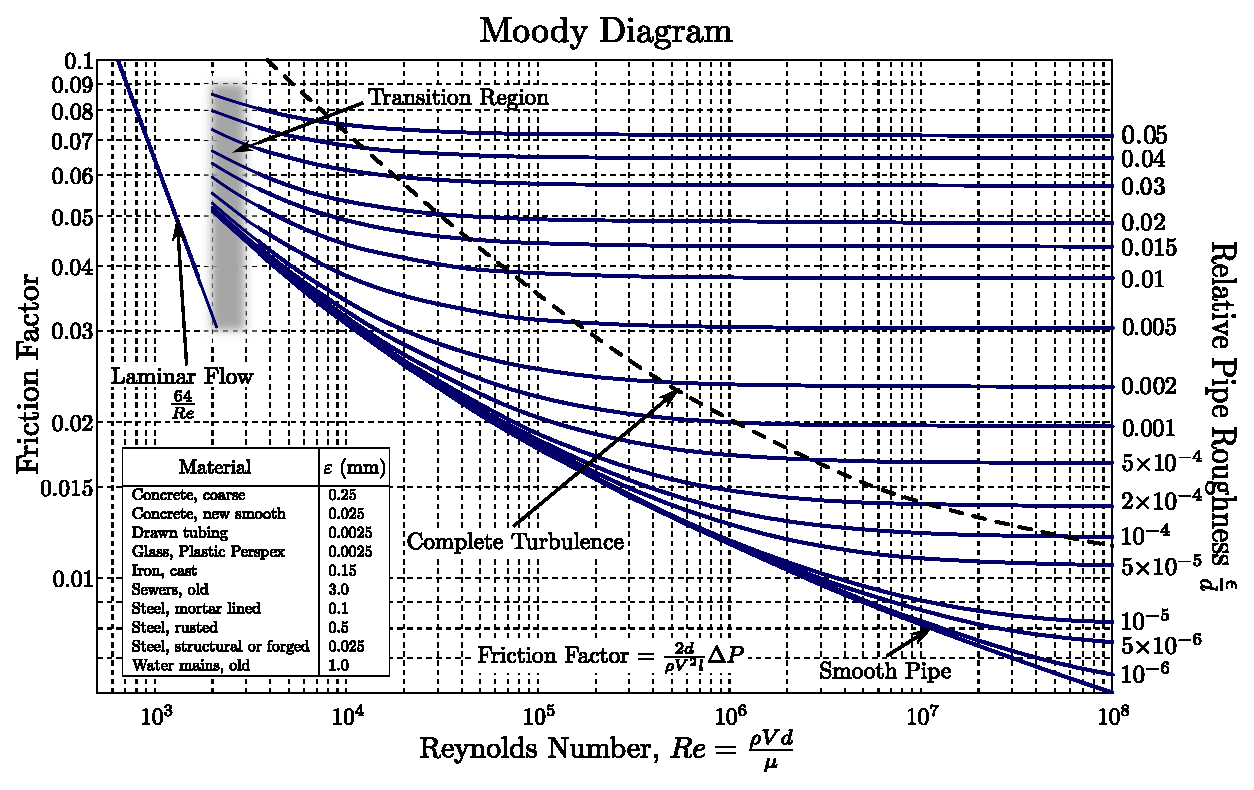
\includegraphics[scale=.75]{img/Moody_EN.eps}
    \caption{Moody chart. {\color{gray}(Wikipedia)}}
    \label{fig:moody}
\end{figure}

\paragraph{Contraction and expansion loss} Energy losses are also associated with expansion/contraction in channel size and bends \textit{etc.} This type of energy loss is known as the \textbf{minor head loss}\footnote{``major'' and ``minor'' do not necessarily reflect the relative importance of each type of loss. The minor loss can be larger than the major loss.}, which leads to the pressure drop
\[
    \Delta p = \rho g h_{f}  \quad \Rightarrow \quad R = \frac{\Delta p}{Q} = \frac{\rho g h_{f} U}{A} = \frac{\rho g K_L U}{2gA}.
\]
where the value of loss coefficient $K_L$ can be found in \autoref{fig:contraction-expansion-losses}. Note that \autoref{fig:contraction-expansion-losses} only applies for the turbulent flow in a pipe $\Rightarrow$ always calculate $\rm Re$ before reading values from the chart!
\begin{figure}[H]
    \centering
    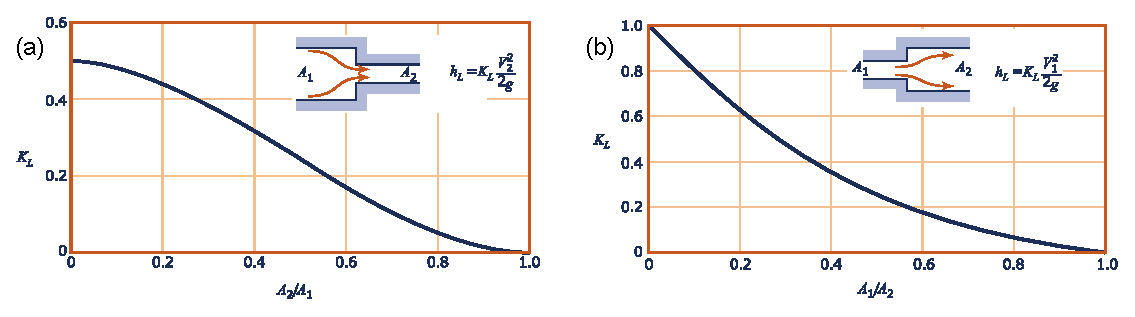
\includegraphics{img/contraction_expansion_loss.eps}
    \caption{Loss coefficient for a sudden (a) contraction, (b) expansion. {\color{gray} (Munson \textit{et al.})}}
    \label{fig:contraction-expansion-losses}
\end{figure}

\vfill
{\small \color{gray}Drafted by B. Li, H. El Nashar, and C. H. Yap,  \today}
% \thispagestyle{empty}
\newgeometry{margin=1.8cm}
\mbox{}
\vfill    
\begin{figure}[H]
    \includegraphics[right]{images/by-nc.eps}
\end{figure}
\textit{This work is licensed under a Creative Commons Attribution-NonCommercial 4.0 International License.}


\end{document}